\clearpage
\appendix
\setcounter{figure}{0}
\renewcommand{\thefigure}{S\arabic{figure}}
\renewcommand{\theHfigure}{supp.\arabic{figure}}
\providecommand{\theHfigurewid}{supp.\arabic{figurewid}}
\section{Verdict fields and review of conflicts}\label{verdict-fields-and-review-of-conflicts}

The lifecycle fields \path{rule_empty}, \path{tcp_failed}, \path{health_ok}, and \path{order_ok} describe the pre-state. The fields \path{new_tcp}, \path{http_ok}, and \path{order_ok} describe the post-state. Together they implement the seven predicates in Section 3.3. When checking the post-state, the native input adapter includes the rule readback and probe order. It compares the target entry with the write parameters using the saved output. Algorithm 1 first checks the feasibility of the entire graph. It reports invalid input, budget exhaustion, and conflicting evidence separately. The \path{must} and \path{may} fields are inapplicable if the target cannot be located or its processing status is unknown. The artifact entries \path{solver-native} and \path{solver-regression} identify the solver entry points.

\section{Native records and window eligibility}\label{native-records-and-window-eligibility}

The \path{native-initial} entry contains the per-window records, eligibility matrix, reference evidence, and per-query results. The six eligible windows were C1-r2, C1-r3, C2-r3, C3-r2, C3-r3, and C4-r3. The \path{native-formal} entry contains the prespecified slots, raw records, eligibility checks, and method comparisons. The \path{native-pilot} entry contains the four engineering pilot windows, including the synchronized case P-C5P. The \path{native-c4-recheck} entry contains three separate rechecks. For the latter three cohorts, \path{audit/reference.json} contains the reference and \path{comparison/records.jsonl} gives the verdict for each query. \path{LEDGER.json} records which windows qualified for the formal cohort.

The Agent was stopped after six seconds in the three formal C4 windows. Event 52007 was recorded, but the end event was missing. All three slots remain in the ledger as ineligible. When the ten-second wait was restored, all three rechecks yielded complete end records. These rechecks diagnose the collection gap and are counted separately from the formal cohort.

The target in C2-r3 is \path{server_knk/3}. KNK transaction 2751184245987731791 is associated with AOP and ART transaction 4699364085620591508. The \path{expired} and \path{after} fields in \path{metadata.json} record the states at expiry and after the write, respectively. Line 338 contains the target rule. In \path{agent.pcap}, packet 16 records the SYN of the failed probe at expiry. Packets 19--30 record the fresh TCP connection and HTTP 200. The health probe at expiry appears in packets 29--40 of \path{control.pcap}. For C1-r2 and C1-r3, line 124 of each \path{metadata.json} gives the post-state rule. Packets 4--15 of each \path{agent.pcap} record the fresh TCP probe.

\section{Synthetic suites and verdict checks}\label{synthetic-suites-and-verdict-checks}

The \path{regression-fixed} artifact contains the development and sealed base instances and the per-instance regression results. The seven additional determinate verdicts occurred on sealed-05, sealed-06, sealed-09, sealed-10, sealed-17, sealed-21, and sealed-22. The \path{synthetic-holdout} artifact contains the frozen inputs for the subsequent 24 instances, the first-run results, and the reference disclosed afterward. \path{VERIFICATION.json} records reconstruction and verification. The archive records the purpose and execution order of each suite separately. The corrected regression rerun belongs to the original suite.

Table~\ref{tab:9} gives the minimum-cardinality deficient sets under Hall's condition for the six prospective synthetic instances on which global queries added a determinate verdict. Each original graph admits a matching that covers every action bundle. After removing the known-success edges to the target request, each minimum-cardinality deficient set contains one more bundle than candidate initiators. The \path{hall-certificates} entry, \path{artifacts/verification/hall_certificates.json}, lists the bundles, candidate initiators, and a matching in the original graph for each instance. The copies were checked against the frozen originals byte for byte and by digest.

\begin{table*}[tbp]

\centering\small

\caption{Minimum-cardinality Hall deficits for the additional determinate verdicts in the prospective sealed suite.}\label{tab:9}

\begin{tabularx}{\textwidth}{@{}rrXX@{}}

\toprule

\textbf{Bundles} & \textbf{Candidate initiators} & \textbf{Capacity exhausted, new admission established} & \textbf{Exchangeable successful bundles, action only} \\

\midrule

4 & 3 & H21 & H19 \\

5 & 4 & H11 & H10 \\

6 & 5 & H05 & H15 \\

\bottomrule

\end{tabularx}

\end{table*}

\section{Archived behavior and evidence index}\label{archived-behavior-and-evidence-index}

The \path{historical-package} entry locates the review package for the initial and archived materials. Items S8--S9 contain the initial native runs. Items S1--S5 index the historical KNK, DRG, and diagnostic records. Appendices B and C cover the later cohorts. The supplementary figures each show their own archived records. Figure~\ref{fig:10} reports the archived KNK receiver and probe results.

\subsection{Sparse records and DRG role checks}\label{sparse-records-and-drg-role-checks}

Processing status was unresolved for seven DRG inputs. Five KNK inputs recorded entry into application processing. The execution effect remained unresolved for both groups. The other four KNK inputs recorded explicit rejection and had no successful target action (Figure~\ref{fig:S1}). Exact enumeration reached its budget on one input. Authorization remained unresolved for all 16 inputs.

\begin{figure*}[tbp]

\centering

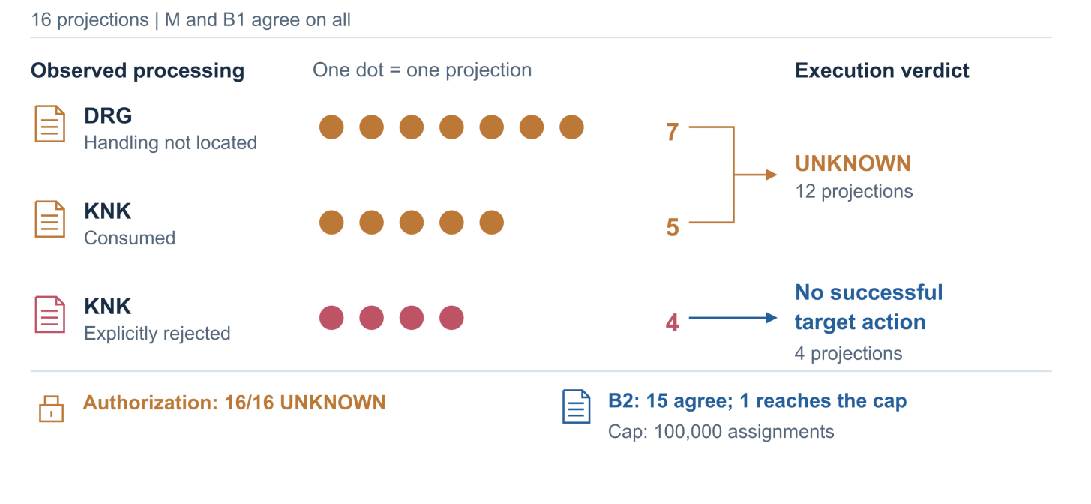
\includegraphics[width=0.94\textwidth,height=0.67\textheight,keepaspectratio]{figures/figS1.pdf}

\caption{Processing status and execution verdicts for inputs with incomplete evidence. Each point denotes one input, and lines link its classifications. The execution effect remained unresolved for seven DRG and five KNK inputs. Four rejected KNK inputs had no successful target action. Authorization and enumeration budget appear separately. ``Cap'' denotes the enumeration limit.}\label{fig:S1}

\end{figure*}

Figure~\ref{fig:S2} shows the DRG writes and role-check results for the DB and static Agent in the initial archive. The role check rejected the Agent request. The records came from two different builds, and the Server send log identifies DAK. The \path{supplement-audit} entry documents the additional controls and configuration-file checks.

\begin{figure*}[tbp]

\centering

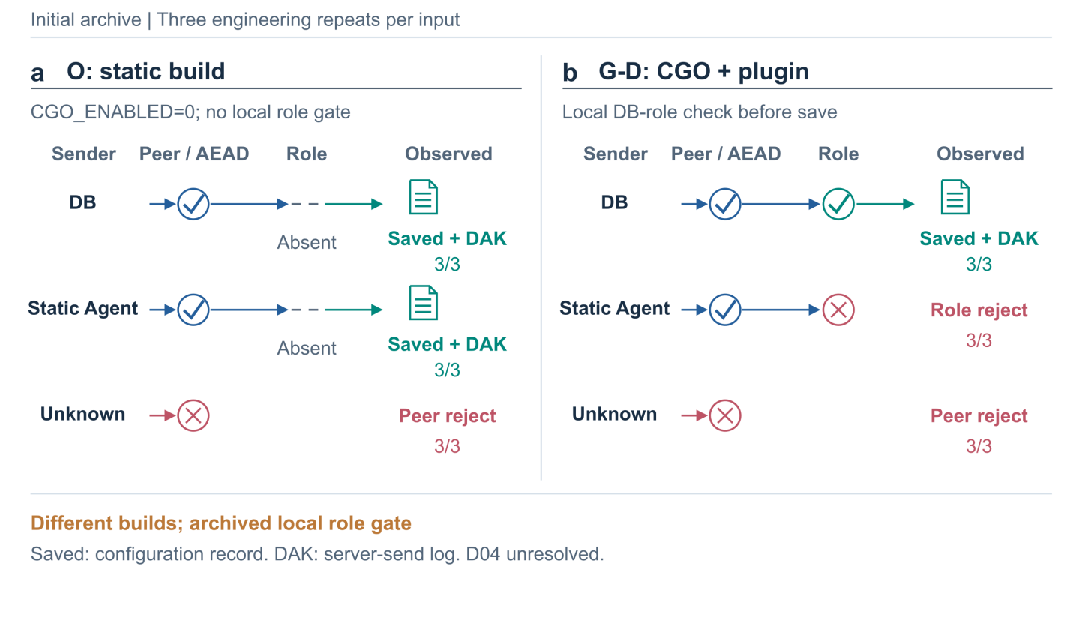
\includegraphics[width=0.94\textwidth,height=0.67\textheight,keepaspectratio]{figures/figS2.pdf}

\caption{DRG checkpoints in the initial archived cohort across two builds. O is the static build. G-D includes a local role check before saving. Each item has three engineering repetitions. The records show configuration creation, and the Server send log identifies DAK. The two arms use different builds.}\label{fig:S2}

\end{figure*}

\subsection{Archived KNK deployment and observation points}\label{archived-knk-deployment-and-observation-points}

Figure~\ref{fig:S3} shows the deployment and observation points for archived cohort S2. A veth pair connected the \path{agentns} (10.0.0.2) and \path{srvns} (10.0.0.1) namespaces. The protected service listened on TCP port 80. C1 and C2 denote UDP connection contexts. Figure~\ref{fig:10} gives receiver and probe outcomes. Figure~\ref{fig:6} shows the TCP port 8080 path used for the native evaluation.

\begin{figure*}[tbp]

\centering

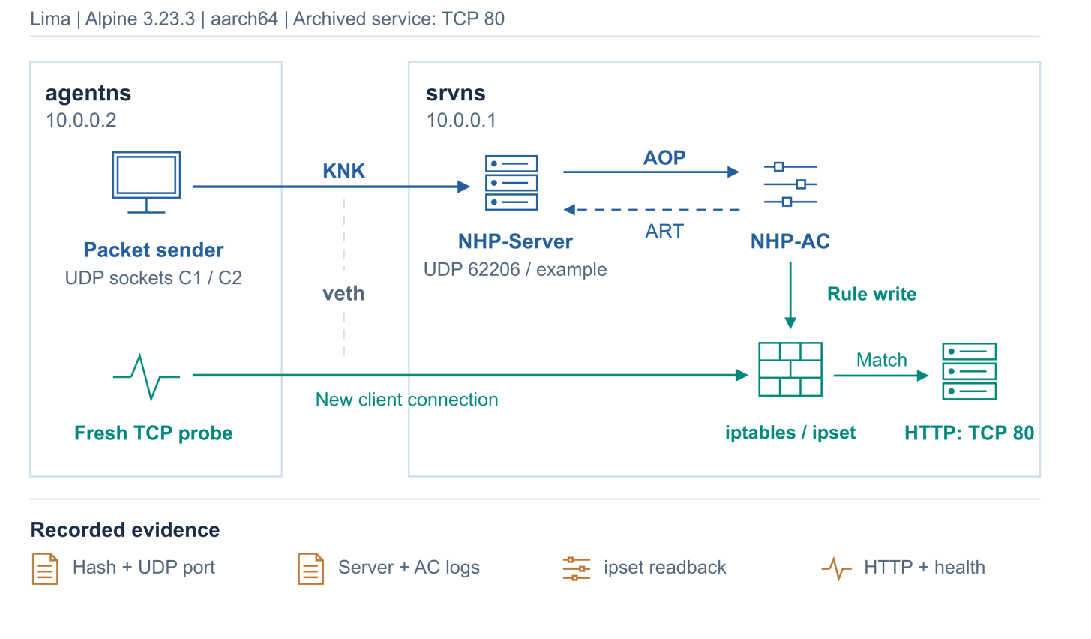
\includegraphics[width=0.94\textwidth,height=0.67\textheight,keepaspectratio]{figures/figS3.pdf}

\caption{Two-namespace deployment for archived cohort S2. C1 and C2 denote UDP sockets, and external probes used TCP port 80. The lower panel lists the record sources. Figure~\ref{fig:6} shows the TCP port 8080 deployment for the native evaluation.}\label{fig:S3}

\end{figure*}

\subsection{Rule expiry and application processing of a previously observed packet}\label{rule-expiry-and-application-processing-of-a-previously-observed-packet}

Figure~\ref{fig:S4} aligns the rule snapshots, AC logs, and TCP/HTTP probes from archived case R02 across the initial knock, expiry check, and subsequent observation. An independent readback showed an empty rule set at expiry. After the previously observed packet was received again, the AC log recorded an execution event, and HTTP 200 over a fresh TCP connection confirmed reachability. The post-state lacked an independent rule readback. The archive distinguishes the period advertised in the acknowledgment from the duration in the recorded control messages and the rule state.

\begin{figure*}[tbp]

\centering

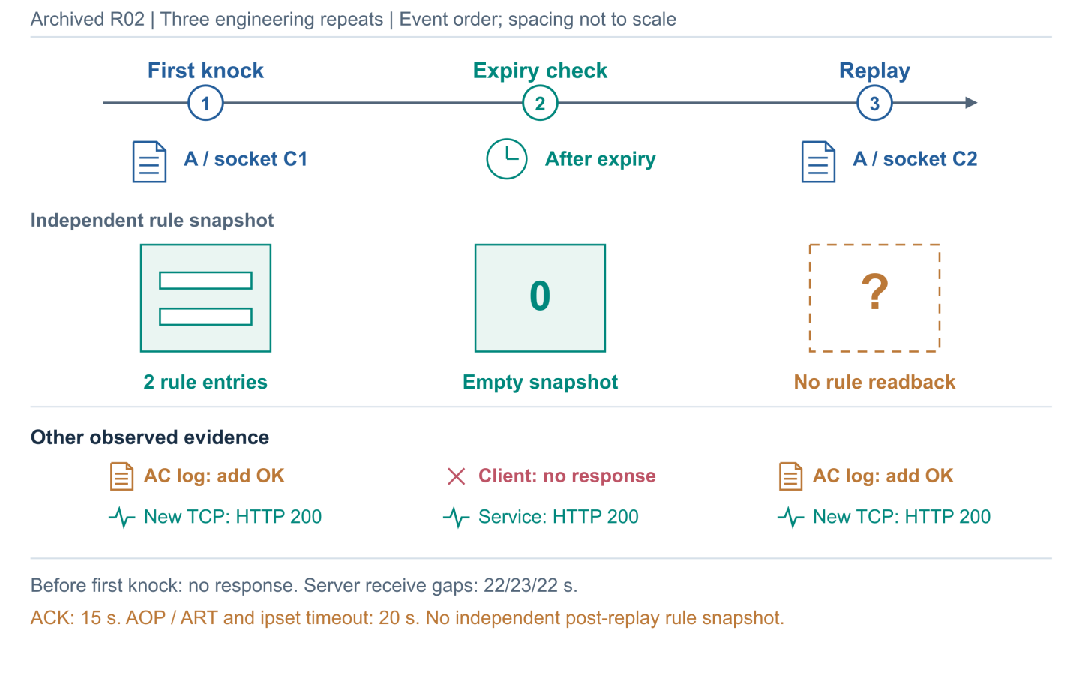
\includegraphics[width=0.94\textwidth,height=0.67\textheight,keepaspectratio]{figures/figS4.pdf}

\caption{Rule snapshots and recorded execution in archived case R02. At expiry, the rule set was empty, the external connection received no response, and the service remained healthy. The later AC log recorded success, and the fresh connection yielded HTTP 200. A question mark denotes the missing independent post-state observation (``No rule readback''). Horizontal position indicates event order only.}\label{fig:S4}

\end{figure*}

\subsection{Execution effects and authorization across interfaces}\label{execution-effects-and-authorization-across-interfaces}

The historical cross-interface diagnostics distinguish effects on protected resources from compliance with authorization rules. For DRG, the measured effect was a write of the data-object registration configuration to a file. For the Console, it was a service configuration change or the registration and initialization of a test helper. For HTTP KBS, it was receipt of an encrypted resource and recovery of the expected plaintext using a test key. These diagnostics are separate from the additional KNK verdict counts.

The diagnostics tested whether adding a handler check prevented the candidate input from triggering a protected operation. Table~\ref{tab:10} reports effects for authorized controls and candidate inputs. Native rejection requirements and the test reference policies are interpreted separately. V2 contained 312 records. Of these, 156 met their respective comparison criteria, comprising 138 main-suite and 18 exploratory records. Table~\ref{tab:10} includes the main-suite cases eligible under every variant of the corresponding interface, covering 14 semantic cases, 40 case--variant cells, and 120 records. Each cell contained three engineering repetitions, and some candidate inputs shared an authorized control.

\begin{table*}[tbp]

\centering\small

\caption{Diagnostic comparison on the common V2 main-suite cases.}\label{tab:10}

\begin{tabularx}{\textwidth}{@{}lXrrr@{}}

\toprule

\textbf{Interface} & \textbf{Variant order} & \textbf{Control effects} & \textbf{Candidate effects} & \textbf{Candidate rejections} \\

\midrule

DRG & Original, harness role check & 3, 3 & 3, 0 & 0, 3 \\

Console & Original, host check only, reference policy & 6, 6, 6 & 12, 12, 0 & 0, 0, 12 \\

HTTP KBS & Original, session check only, reference policy & 3, 3, 3 & 15, 9, 0 & 0, 6, 15 \\

\bottomrule

\end{tabularx}

\end{table*}

The harness role check prevented the static Agent's DRG write. Whether the receiver is required to reject the request depends on the applicable rule. The harness set the caller identity for the Console. In the shared cases where the host condition held, the added host check left the candidate effects unchanged. An authorized configuration in which the host condition was false failed in three additional runs of that variant. For HTTP KBS, the session check reduced deviations from the test reference policy. The reference variant also checked the binding between the synthetic evidence and the key. The exploratory cross-resource case added three deviations to each of the original and session-check-only variants.

\section{Security and performance verification artifacts}\label{security-and-performance-verification-artifacts}

The \path{model-verification} artifact contains the security-model checks. \path{PROTOCOL.md} and \path{FREEZE.json} specify the frozen input domain and implementation. \path{MODEL_RECORDS.jsonl} records the input hashes and six-field output signatures for 26,880 inputs. \path{RESULTS.json} summarizes the results. \path{ASSUMPTION_CONTROLS.json} contains six classes of assumption controls and their enumeration witnesses. \path{NATIVE_EVIDENCE.json} contains the raw JSON, log lines, and hashes for 18 archived KNK records. A read-only verifier reconstructs inputs and checks signatures and artifact hashes without rerunning the product experiments.

The \path{network-performance} artifact contains the network-cost measurements. \path{FREEZE.json} specifies the formal order, scripts, and build. \path{FORMAL_LEDGER.json} records the 80 formal windows. The raw records contain process identities, timings, rule readbacks, event records, and packet captures for each window. \path{RESULTS.json} and \path{records.csv} report the metrics and within-block comparisons. \path{SEAL.json} records their hashes. The v1 preflight had two startup failures without timing data. One of its four completed windows had packet-capture loss. The four windows in the revised Q0 preflight are kept separate from the formal statistics.

The \path{offline-performance} artifact contains the prespecified block order, call and resource records for 480 invocations, and per-instance agreement checks. The \path{figure-rebuild} entry indexes the frozen inputs, SVG and PDF files, per-figure data, and input and output hashes for Figures 8, 9, and 11--13. By default, \path{scripts/plot_figures.py} checks provenance. An explicit redraw invokes the original generators with their original path-resolution behavior. The original plotting scripts, frozen records, and older sealed packages remain at their original locations. The performance and model-verification analyses use separate units and denominators.
